\documentclass{article}


%% We should use this latex document to store all the figures and
%% tables, and then do "make" to generate the floats.pdf which we will
%% send along with the main manuscript text.
\usepackage[a4paper,margin=2cm]{geometry}
\usepackage{graphicx}
\usepackage{mathpazo}

\begin{document}
\pagestyle{empty}


%% One float per page:
%% http://tex.stackexchange.com/questions/22191/forcing-a-figure-strictly-on-a-separate-page
\makeatletter
\@fpsep\textheight
\makeatother

\begin{figure}
  \centering
  \fbox{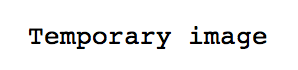
\includegraphics{temp.png}}
  \caption{Example raster plot from one well over the four DIV
studied. Each row represents the spike train from one electrode. The
scale bar for all raster plots is 60s.}
\end{figure}

\begin{figure}
  \centering
  \fbox{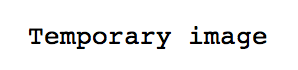
\includegraphics{temp.png}}
  \caption{A Firing rate, and B within burst firing rate.}
\end{figure}

\begin{figure}
  \centering
  \fbox{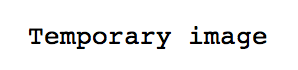
\includegraphics{temp.png}}
  \caption{A Fraction of bursting electrodes, B bursts per minute, C
burst duration, D percentage of spikes in bursts, E CV of IBI, and F
CV of within burst ISI.}
\end{figure}

\begin{figure}
  \centering
  \fbox{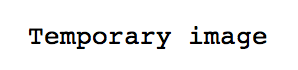
\includegraphics{temp.png}}
  \caption{A Network spike rate, B network spike peak, C network spike
duration, and D mean correlation.}
\end{figure}

\begin{figure}
  \centering
  \fbox{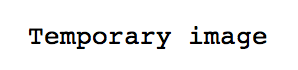
\includegraphics{temp.png}}
  \caption{[Top left] Well-level PCA projection of 12-dimensional
feature vectors onto PC dimension 1 (x-axis) and 2 (y-axis).  Each dot
represents a well, colored by day in vitro (DIV) of recording. Rough
ordering from youngest (lightest, DIV 5) to oldest (darkest, DIV 12)
wells is apparent in darkening of colors along the positive direction
. (Top right) Scree plot displays \% variance explained by the number
of PC dimensions. [Bottom left] Plate-level PCA projection of plate
averages onto PC dimension 1 (x-axis) and 2 (y-axis).  As in top,
rough ordering of observations by DIV is apparent in the light to dark
transition along the x-axis. (Bottom right) Scree plot of plate-level
PCA. Compared to the well-level PCA scree plot, a larger amount of
variation is captured in the first two PC dimensions indicating that
well averaging reduces variability.
}
\end{figure}

\begin{figure}
  \centering
  \fbox{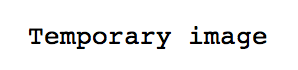
\includegraphics{temp.png}}
  \caption{Average importance of features in driving classification,
    relative to the most important feature.}
\end{figure}

\begin{table}
  \centering
  \caption{Features used in our analysis and a brief description of how
    they were calculated.}
\end{table}

\begin{table}
  \centering
  \caption{Classifier performance at predicting the age of
arrays. Features are listed in decreasing order of importance, and the
value in each row n=1,...,12 is the mean percentage of correct
classifications using the top n features.}
\end{table}

\begin{table}
  \centering
  \caption{Classifier performance at predicting the age of arrays for
    each pairwise combination of DIV. Features are listed in
    decreasing order of importance, and the value in each row
    n=1,...,12 is the mean percentage of correct classifications using
    the top n features.}
\end{table}



\end{document}
